% Copyright 2021  Stefano Fochesatto

\documentclass[xcolor={svgnames},
               hyperref={colorlinks,citecolor=DeepPink4,linkcolor=FireBrick,urlcolor=Maroon}]
               {beamer}

\mode<presentation>{
  \usetheme{Berlin}
  \usecolortheme{orchid}
  \setbeamercovered{transparent}
  \setbeamerfont{frametitle}{size=\large}
}
\usetheme[headline,footline]{UAFblue}
\setbeamercolor*{block title}{bg=red!10}
\setbeamercolor*{block body}{bg=red!5}

\usepackage[english]{babel}
\usepackage[latin1]{inputenc}
\usepackage{times}
\usepackage[T1]{fontenc}
% Or whatever. Note that the encoding and the font should match. If T1
% does not look nice, try deleting the line with the fontenc.

\usepackage{empheq,bm}
\usepackage{xspace}
\usepackage{fancyvrb}

\usepackage{tikz}
\usetikzlibrary{shapes,arrows.meta,decorations.markings,decorations.pathreplacing,fadings,positioning}

\usepackage[kw]{pseudo}
\pseudoset{left-margin=15mm,topsep=5mm,idfont=\texttt,st-left=,st-right=}


% If you wish to uncover everything in a step-wise fashion, uncomment
% the following command:
%\beamerdefaultoverlayspecification{<+->}

\newcommand{\ba}{\mathbf{a}}
\newcommand{\bb}{\mathbf{b}}
\newcommand{\bc}{\mathbf{c}}
\newcommand{\bbf}{\mathbf{f}}
\newcommand{\bg}{\mathbf{g}}
\newcommand{\bn}{\mathbf{n}}
\newcommand{\bq}{\mathbf{q}}
\newcommand{\br}{\mathbf{r}}
\newcommand{\bx}{\mathbf{x}}
\newcommand{\by}{\mathbf{y}}
\newcommand{\bv}{\mathbf{v}}
\newcommand{\bu}{\mathbf{u}}
\newcommand{\bw}{\mathbf{w}}

\newcommand{\bF}{\mathbf{F}}
\newcommand{\bG}{\mathbf{G}}
\newcommand{\bQ}{\mathbf{Q}}

\newcommand{\grad}{\nabla}
\newcommand{\Div}{\nabla\cdot}
\newcommand{\minmod}{\operatorname{minmod}}

\newcommand{\CC}{\mathbb{C}}
\newcommand{\RR}{\mathbb{R}}

\newcommand{\ddt}[1]{\ensuremath{\frac{\partial #1}{\partial t}}}
\newcommand{\ddx}[1]{\ensuremath{\frac{\partial #1}{\partial x}}}
\newcommand{\Matlab}{\textsc{Matlab}\xspace}
\newcommand{\Octave}{\textsc{Octave}\xspace}
\newcommand{\eps}{\epsilon}

\newcommand{\ip}[2]{\left<#1,#2\right>}

\newcommand{\xiphalf}{{x_{i+\frac{1}{2}}}}
\newcommand{\ximhalf}{{x_{i-\frac{1}{2}}}}
\newcommand{\Fiphalf}{{F_{i+\frac{1}{2}}}}
\newcommand{\Fimhalf}{{F_{i-\frac{1}{2}}}}
\newcommand{\Fiphalfn}{{F^n_{i+\frac{1}{2}}}}
\newcommand{\Fimhalfn}{{F^n_{i-\frac{1}{2}}}}

\newcommand{\trefcolumn}[1]{\begin{bmatrix} \phantom{x} \\ #1 \\ \phantom{x} \end{bmatrix}}
\newcommand{\trefmatrixtwo}[2]{\left[\begin{array}{c|c|c} & & \\ #1 & \dots & #2 \\ & & \end{array}\right]}
\newcommand{\trefmatrixthree}[3]{\left[\begin{array}{c|c|c|c} & & & \\ #1 & #2 & \dots & #3 \\ & & & \end{array}\right]}
\newcommand{\trefmatrixgroups}[4]{\left[\begin{array}{c|c|c|c|c|c} & & & & & \\ #1 & \dots & #2 & #3 & \dots & #4 \\ & & & & & \end{array}\right]}

\newcommand{\blocktwo}[4]{\left[\begin{array}{c|c} #1 & #2 \\ \hline #3 & #4 \end{array}\right]}

\newcommand{\bqed}{{\color{blue}\qed}}
\newcommand{\ds}{\displaystyle}

\newcommand\mynum[1]{{\renewcommand{\insertenumlabel}{#1}%
      \usebeamertemplate{enumerate item} \,}}


\title{Decision Tree Learning from Scratch}

\author{Stefano Fochesatto}

\institute[UAF]{MATH 692 Mathematics for Machine Learning}

\date[Spring 2022]{2/10/2022}

%\titlegraphic{\begin{picture}(0,0)
%    \put(0,180){\makebox(0,0)[rt]{\includegraphics[width=4cm]{figs/software.png}}}
%  \end{picture}
%}

%% this nonsense needed to start section counter at 0; see
%% https://tex.stackexchange.com/questions/170222/change-the-numbering-in-beamers-table-of-content
\makeatletter
\patchcmd{\beamer@sectionintoc}
  {\ifnum\beamer@tempcount>0}
  {\ifnum\beamer@tempcount>-1}
  {}
  {}
%\beamer@tocsectionnumber=-1
\makeatother


\begin{document}
\beamertemplatenavigationsymbolsempty

\begin{frame}
  \maketitle
\end{frame}

\begin{frame}{Presentation Outline}
  \begin{itemize}
  \item What is a Decision Tree?
  \vfill
  \item Motivations and Prevalence.
  \vfill
  \item Training the Tree.
  \vfill
  \item Advantages and Pitfalls.
  \vfill
  \item Code Demo.
  \vfill
  \item Application in Ensemble Models.
  \end{itemize}
\end{frame}







\begin{frame}{What is Decision Tree Learning?}
    \begin{columns}[T]
      \begin{column}{.60\textwidth}
        \begin{center}
        \begin{itemize}
            \item Supervised Learning.  
            \item A flowchart where internal nodes represent a test for the data.
            \item Leaf nodes apply classification label or regression.
            \item Derived from recursive partitioning. 
            \item We will discuss classification mainly, 
        \end{itemize}
      \end{center}
      \end{column}
      \begin{column}{.50\textwidth}
            \begin{figure}
              \vspace*{\fill}
              \begin{center}
            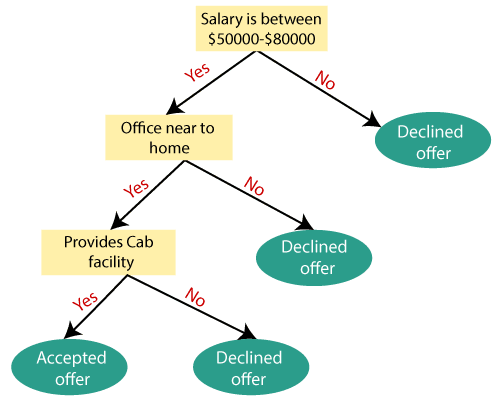
\includegraphics[width=.75\textwidth]{ExampleTree.png}
          \caption{Decision Tree Example}
              \end{center}
              \vspace*{\fill}
            \end{figure}
          \end{column}
    \end{columns}
  \end{frame}

  \begin{frame}{What is Decision Tree Learning?}
            \begin{figure}
              \vspace*{\fill}
              \begin{center}
            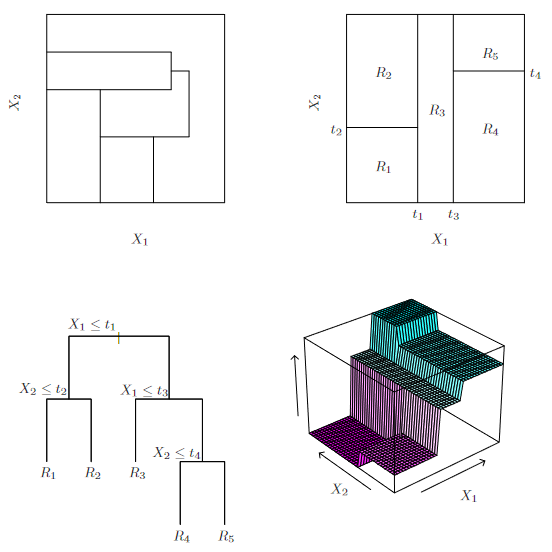
\includegraphics[width=.55\textwidth]{ESLDecisionTreeExample.png}
          \caption{E.S.L. Friedman, Hastie, Tibshirani}
              \end{center}
              \vspace*{\fill}
            \end{figure}
  \end{frame}


  
  \begin{frame}{Training the Tree.}
    \begin{itemize}
    \item Methods don't guarantee the optimal solution (Greedy). 
    \vfill
    \item Top-Down Induction of Decision Trees (R.Quinlan)
    \vfill
    \item There are several algorithms for training.
      \begin{itemize}
        \item CART (L.Breimann)
        \item ID3 and C4.5 (R.Quinlan)
        \item C5.0 (R.Quinlan)
      \end{itemize}
    \end{itemize}

  \end{frame}

  
  \begin{frame}{Information Theory}
    \begin{itemize}
      \item Consider the following splits,
      \begin{columns}[T]
        \begin{column}{.45\textwidth}
          \begin{figure}
            \vspace*{\fill}
            \begin{center}
          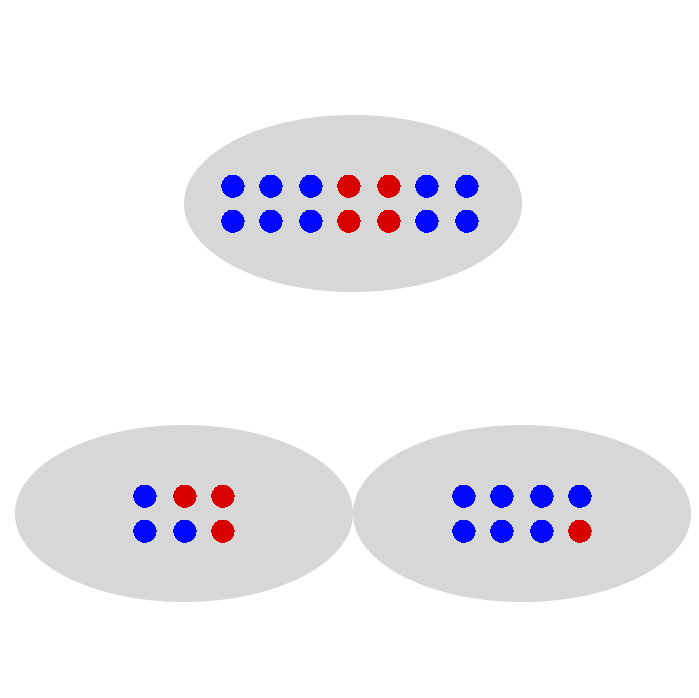
\includegraphics[width=.85\textwidth]{HighEntropy.png}
        \caption{Example Split \# 1}
            \end{center}
            \vspace*{\fill}
          \end{figure}
        \end{column}
        \begin{column}{.45\textwidth}
              \begin{figure}
                \vspace*{\fill}
                \begin{center}
              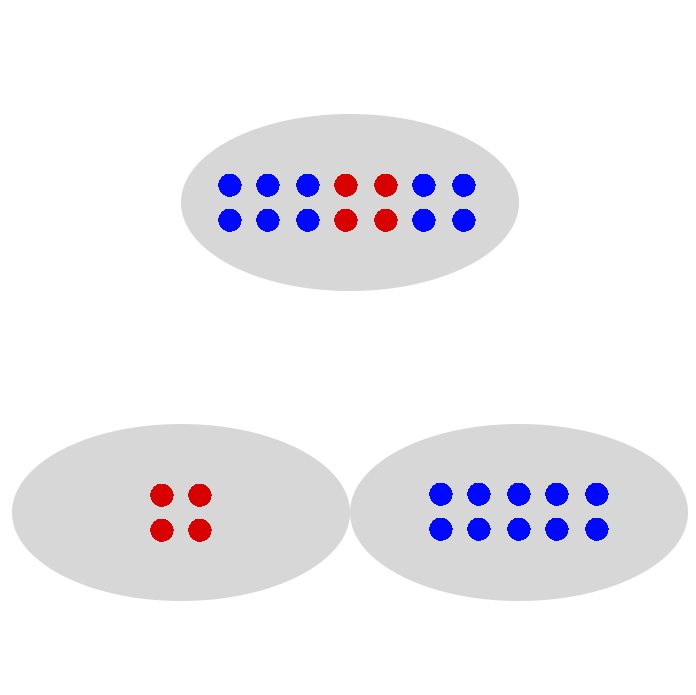
\includegraphics[width=.85\textwidth]{LowEntropy.png}
            \caption{Example Split \# 2}
                \end{center}
                \vspace*{\fill}
              \end{figure}
            \end{column}
      \end{columns}
      \item To optimize our tree we need to be able to quantify the quality of a split (or generalized state)?
    \end{itemize}  
  \end{frame}


  \begin{frame}{Information Theory}
    \begin{itemize}
      \item Let $X$(observation) be a discrete random variable with $n$(classes) possible outcomes and pmf p(x)(prob distribution at node).
      \vfill
      \item In information theory, the unit of information ascribed to an outcome $x \in n$ is a log measure of 1/p(x),
      \begin{equation*}
        I = \log\left(\frac{1}{p(x)}\right) = -\log(p(x)).
      \end{equation*} 
      \vfill
      \item Events that are rare have more information, events that are common have less information. 
    \end{itemize}
  \end{frame}

  \begin{frame}{Information Theory}
    \begin{itemize}
      \item We want to know the expected information at a node over all outcomes (classification classes), 
      \begin{equation*}
        \mathbb{E}(I) = \sum_{i = 1}^n p(i) \log_2\left(\frac{1}{p(i)}\right) = -\sum_{i = 1}^n p(i)\log_2(p(i)).
      \end{equation*}
      \vfill
      \item We want to find the split which maximizes $\Delta I$ or information gain, 
      \begin{equation*}
        \Delta I = \mathbb{E}(I)_{Parent} - \sum w(i) \mathbb{E}(I)_{Children}.  
      \end{equation*}
      \item Where $w(i)$ is the size of the child node relative to the parent node. 
      \vfill
      \item Sometimes we only care about the difference between splits. 
      \begin{equation*}
        \Delta I = 1 - \sum w(i) \mathbb{E}(I)_{Children}.  
      \end{equation*}
    \end{itemize}
  \end{frame}


  \begin{frame}{Training the Tree}
    \begin{itemize}
    \item For the CART algorithm the Gini Impurity is used to evaluate the quality of a node, 
    \begin{equation*}
      Gini = 1 - \sum_{i = 1}^n p(i)^2.
    \end{equation*}
    \item Again evaluating a split we take a weighted sum, 
    \begin{equation*}
      Gini_{split} = \sum Gini_{children}.
    \end{equation*}
    \item Both methods are largely the same, Gini is preferred for predictive performance and computational complexity. 
  \end{itemize}
  \end{frame}

  \begin{frame}{Training the Tree}
  \begin{itemize}
     \item BuildTree(node);
     \begin{itemize}
       \item if statement for stopping criteria;
       \item Best\_gini = gini(node.observations)
       \item Best\_feature
       \item Best\_threshold
       \item loop through features;
       \begin{itemize}
         \item sort all observations by current feature;
         \item loop through observations;
         \begin{itemize}
           \item left\_gini = gini(node.observations[1:i])
           \item right\_gini = gini(node.observations[i+1:n])
           \item split\_gini = (i/n)left\_gini + ((i+1 - n)/n)right\_gini
           \item if split\_gini < Best\_gini; Best\_Gini = split\_gini; Best\_feature = j; Best\_threshold = i
         \end{itemize}  
       \end{itemize}
       \item BuildTree(node.left)
       \item BuildTree(node.right)
      \end{itemize}
    \end{itemize}
  \end{frame}




\end{document}